% !TeX root=../main.tex

\chapter{مقدمه}
% دستور زیر باعث عدم‌نمایش شماره صفحه در اولین صفحهٔ این فصل می‌شود.
%\thispagestyle{empty}
\section{معرفی ویژگی‌های متمایزکننده‌ی شبکه‌ی اینترنت اشیا}
رشد شبکه‌های اینترنت اشیا کاربردهای زیادی از جمله سیستم پایش سلامت \footnote{\lr{health-care system}}،‌ خانه‌ی هوشمند \footnote{\lr{smart home}} و شهر هوشمند \footnote{\lr{smart city}}را توسعه بخشیده است. بخش زیربنایی کاربردهای مبتنی بر شبکه‌های اینترنت اشیا، اندازه‌گیری و گزارش دیتاهایی مانند دما، رطوبت، ویدیو و ... می‌باشد. این اطلاعات از طریق درگاه‌\footnote{gateway}ها به گره‌های مصرف کننده می‌رسد. افزایش تعداد گره‌های مصرف کننده و نیز تعداد حسگرها ترافیک عظیمی در شبکه‌های اینترنت اشیا ایجا کرده و نیز میزان تراکم در این شبکه‌ها را بالا می‌برد. این مسئله باعث کاهش میزان کیفیت سرویس می‌شود. به علاوه اینکه فعالسازی دوباره‌ی حسگرها برای واکشی پاسخ، میزان انرژی مصرفی آنها را بالا برده و از عمر باتری آنها کم می‌کند.

شبکه‌های اینترنت اشیا دارای دو ویژگی متمایز و چالش‌زا می‌باشند. اول اینکه تأمین انرژی اکثر تجهیزات و حسگرها از طریق باتری تأمین می‌شود و بنابراین با انرژی محدود کار می‌کنند و بالا بودن حجم درخواست‌ها باعث می‌شود تا از دست دادن انرژی در آنها سریعتر رخ دهد. دوم اینکه دیتای گزارش شده توسط حسگرها برای مدت زمان کوتاهی معتبر یا به عبارتی تازه می‌باشد و پس از مدتی منقضی می‌شود. در بعضی از مقالات به ویژگی دوم تحت عنوان تازگی دیتا\footnote{\lr{data freshness}} و در بعضی دیگر تحت یک مفهوم کلی تر با نام سن اطلاعات\footnote{\lr{Age of Information (AoI)}} اشاره شده است. 
\subsection{استراتژی ذخیره‌سازی}
حال ذخیره سازی به عنوان راه حلی برای متوازن‌سازی ترافیک در شبکه مطرح می‌شود به این معنا که در درگاه‌های شبکه‌های اینترنت اشیا یک حافظه‌ی ذخیره‌سازی قرار گرفته است که اطلاعات را جمع‌آوری می‌کند و می‌تواند به طور موقت دیتا را ذخیره کرده و در صورت ارسال درخواست از سوی گره‌های مصرف کننده، دیتای مربوطه را برای آنها بفرستد. 

در سناریوی توصیف شده از ارتباط مستقیم لینک‌های پشتی\footnote{\lr{backhaul links}} با حسگرها جلوگیری کرده‌ایم که در اثر آن ترافیک شبکه معادلتر شده و حجم درخواست‌های ارسالی به یک حسگر کاهش می‌یابد و بنابراین حسگر به تعداد دفعات کمتری برای واکشی پاسخ فعال می‌شود و مصرف انرژی در آن کاهش‌ می‌یابد. در سناریوی مطرح شده باید قیدی را مبنی بر محدودیت حافظه‌ی ذخیره‌سازی در نظر داشته باشیم به علاوه‌ی اینکه به طراحی یک سیاست مناسب برای ذخیره‌سازی محتوا با در نظر گرفتن فاکتور تازگی دیتا نیاز داریم.  

تعداد قابل توجهی از تحقیقات تا قبل از سال 2018 به یک استراتژی ذخیره‌سازی مبتنی بر محتوا\footnote{\lr{ICN caching}} برای یک نیاز خاص در شبکه‌های اینترنت اشیا پرداخته‌اند و روش‌هایی را مبتنی بر طبیعت \lr{ad-hoc} و بی‌سیم شبکه‌های اینترنت اشیا ارائه کرده‌اند. 

عموماً یک استراتژی ذخیره‌سازی می‌تواند بر دو جنبه اثر بگذارد: یکی اینکه کدام محتوا در حافظه‌ی کش ذخیره گردد که به عبارتی به تصمیم برای ذخیره‌ی محتوا\footnote{\lr{caching decision}} می‌پردازد و دیگری آنکه در صورتیکه ظرفیت حافظه‌ی کش پر شود، الویت با حذف کدام یک از محتواها می‌باشد و یا به عبارتی مکانیزم یا سیاست جایگزینی محتوا\footnote{\lr{cache replacement policy}} را تحت تأثیر قرار می‌دهد. 

\subsubsection{\lr{LCE(Leave Copy Everywhere)}}
سر راست ترین استراتژی ذخیره‌سازی \lr{CEE} یا به تعبیری \lr{LCE (Leave Copy Everywhere)} می‌باشد. در این حالت تمامی گره‌های مسیر برای ذخیره‌سازی محتوای ورودی تلاش می‌کنند. در شبکه‌های مرسوم مبتنی بر محتوا، با توجه به این موضوع که به طور پیش‌فرض محتوا حجم زیادی دارد، این روش با اغماض قابل قبول بوده و سربار کمی نیز ایجاد می‌کند و برتری اصلی آن در اینست که سریعترین انتشار ممکن از محتوا را پیشنهاد می‌دهد.

در این استراتژی گره‌های مسیر هر محتوایی را که شنود می‌کنند، بلافاصله در حافظه ذخیره می‌نمایند. این مسئله وجود کپی از محتوا را تضمین می‌نماید ولی باعث می‌شود تا بیش از حد مورد نیاز کپی از آن محتوا وجود داشته باشد در حالیکه از قابلیت‌ها و منابع شبکه به درستی استفاده نکرده‌ایم. عملاً یکی از اهداف در این مسئله کاهش موارد زائد و بالا بردن تنوع می‌باشد یعنی انتظار داریم تا در حافظه‌های مختلف، چینش‌های متفاوتی از محتواهای موجود ذخیره شده باشند. 
\subsubsection{\lr{ProbCache caching}}
دو پیاده‌سازی استاتیک و دینامیک برای این استراتژی ذخیره‌سازی وجود دارد. در استراتژی استاتیک، یک مقدار ثابت \lr{p} و بتبع بین 0 و 1 برای احتمال ذخیره سازی در گره‌های مسیر درنظر گرفته می‌شود. با گذر محتوای جدید از هر گره در مسیر، آن گره یک عدد رندوم تولید کرده و در صورتیکه این مقدار از \lr{p} کمتر باشد، محتوا را ذخیره می‌کند و در غیر اینصورت آن را تنها جلو می‌راند. 

در این شرایط محتوای محبوب تر که در طول زمان با نرخ بیشتری درخواست می‌شود،‌ شانس بالاتری برای ذخیره سازی پیدا می‌کند. در واقع احتمال ذخیره‌سازی محتوا بعد از \lr{n} بار دریافت شدن به صورت $1-(1-p)^n$ محاسبه می‌شود که با افزایش \lr{n} این مقدار به 1 میل می‌کند. یعنی هر چه میزان محبوبیت فایل یا محتوا بیشتر باشد، احتمال ذخیره‌ی آن نیز افزایش می‌یابد. 

در حالت دینامیک احتمال ذخیره کردن محتوا در یک گره براساس پارامترهایی مانند تازگی،‌ نوع یا تولیدکننده‌ی محتوا، میزان سطح انرژی گره، توپولوژی شبکه و گره های مجاور آن و یا سایر اطلاعات محلی ایجاد می‌گردد.

\subsubsection{\lr{Betweenness Centrality Caching}}
در این استراتژی پارامتری براساس توپولوژی شبکه برای هر گره محاسبه می‌شود. درواقع تعداد بارهایی که آن گره در مسیرهایی بین فرستده و گیرنده قرار می‌گیرد، محاسبه شده و بسته به توپولوژی در جایی که این پارامتر بیشینه می گردد،‌ یک کپی از محتوا ذخیره می‌شود.

\subsubsection{\lr{LCD(Leave Copy Down)}}
در این استراتژی ذخیره‌سازی یک کپی و آن هم در نزدیکترین گره به سنسور، یعنی در درگاه متصل به سنسور قرار داده می‌شود. در این حالت کپی‌های زائد از محتوای مدنظر در سایر گره‌ها قرار ندارد، درواقع نسبت به حالت‌های قبلی از این حیث استفاده‌ی بهینه‌تری از منابع کرده‌ایم اما همچنان برای واکشی پاسخ، درخواست ارسال شده تا گره یکی مانده به سنسور بالا می‌رود که این مسئله چندان مطلوب نیست.

\subsubsection{\lr{Edge Caching}}
در استراتژی ذخیره‌سازی لبه مانند حالت \lr{LCD} یک کپی از محتوا ولی دقیقاً در خلاف جهت آن یعنی در نزدیکترین گره به مصرف کننده یا در دستگاه کاربر ذخیره می‌گردد که عملاً مشکل حالت قبلی در اینجا رفع شده است یعنی درخواست برای واکشی پاسخ تا حسگر یا گره‌های نزدیک به آن بالا نمی‌رود و عملاً ازحجم ترافیک شبکه کم می‌شود.

\paragraph{}
در شکل \ref{fig:cachingStrategy} استراتژی‌های متداول در شبکه‌های مبتنی بر محتوا را (که پیشتر به آنها اشاره شد،) مشاهده می‌کنید.
\begin{figure}[ht]
	\centerline{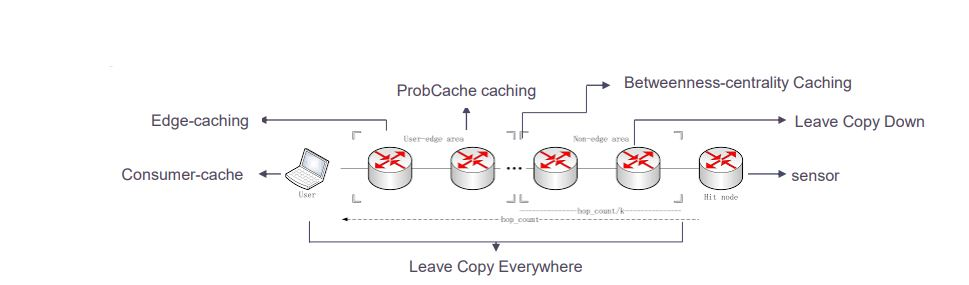
\includegraphics[width=13cm]{cachingStrategy}}
	\caption{استراتژی های متداول ذخیره‌سازی در شبکه‌های مبتنی بر محتوا برگرفته از\\ \lr{\href{https://mdpi-res.com/d_attachment/futureinternet/}{future internet}}}
	\label{fig:cachingStrategy}
\end{figure}

\subsection{سیاست جایگزینی محتوا}
در عمل به دلیل سایز محدود حافظه‌ی ذخیره‌سازی به یک سیاست مناسب برای جایگزینی محتوا در حافظه نیاز داریم. درواقع اصلی ترین هدف ما، یافتن بهینه ترین سیاست در تعامل با محیط می‌باشد به گونه‌ای که میزان تأخیر در ارسال دیتا برای یک محتوا را کمینه نماید.

  قطعاً استراتژی ذخیره‌سازی برای بعضی از محتویات که در طول زمان هیچ درخواستی برای آنها در شبکه وجود ندارد‌ و قبل از انتظار ما برای برآوردن درخواست دیتای مربوط به آنها منقضی می‌شود، مطلوب ما نیست. به عبارتی می توان گفت که در این حالت یک سیاست جایگزینی محتوای مناسب به کارایی استراتژی ذخیره‌‌سازی انتخاب شده، ‌کمک خواهد کرد. یک سری روش رایج جایگزینی برای شبکه‌های \lr{NDN} تعریف گردیده است که برجسته‌ترین و قدیمی‌ترین سیاست مطرح شده، \lr{FIFO (First Input, First Output)} می‌باشد.
  
  سیاست‌های جایگزینی مرسوم،‌ به چهار دسته مطابق با جدول\eqref{tab:replacementPolicies} تقسیم می‌گردند که در ادامه به آنها می‌پردازیم.
  \begin{table}[ht]
  	\caption{سیاست‌های مرسوم برای جایگزینی محتوا}
  	\label{tab:replacementPolicies}
  	\centering
  	\onehalfspacing
  	\begin{tabular}{|r|c|l|r|}
  		\hline \lr{Existing Plicies} & \lr{Description} & \lr{Category} \\ 
  		\hline \lr{LRU, LRU-threshold,} & \lr{Keeps the recently referenced objects} & \lr{Recency-based} \\
  			   \lr{LRU-hot, SLRU,} & \lr{} & \lr{} \\ 
  			   \lr{HLRU, LRU-LSC} & \lr{} & \lr{} \\ 
  		\hline \lr{LFU, LFU-Aging,} & \lr{Keeps the most requested objects} & \lr{Frequency-based} \\ 
  			\lr{LFU-DA, swLFU} & \lr{} & \lr{} \\
  		\hline \lr{RR, RAND,} & \lr{A simple random choice} & \lr{Randomized Policies} \\ 
  		\lr{HARMONIC} & \lr{to avoid computation overhead} & \lr{} \\
  		\hline \lr{SIZE, PSS, CSS} & \lr{Evicts large contents} & \lr{Size-based} \\ 
  		\hline 
  	\end{tabular} 
  \end{table}
  
  \subsubsection{\lr{Recency-Based Replacement Policies}}
  معروف‌‌ترین و پرکاربردترین سیاست از میان سیاست‌های جایگزینی محتوا در این دسته، سیاست \lr{LRU(Least Recently Used)} می‌باشد. (می توان گفت که سایر سیاست‌های متعلق به این دسته از سیاست \lr{LRU} مشتق شده‌اند.) در این حالت هریک از گره‌ها مجموعه‌ی درخواست‌های ارسال شده برای هریک از محتوا را دنبال می‌کند و زمانیکه نیاز به جایگزینی محتوا برای ذخیره‌ی محتوای جدید باشد، محتوایی را که اخیراً از آن کمتر از سایرین استفاده شده است را از حافظه دور می‌ریزد و فایل جدید را ذخیره می‌کند. روش مطرح شده نسبت به سایر سیاست‌های جایگزینی، کارایی بسیار بالایی دارد، اما در شرایطی که تعداد محتویات محبوب از سایز حافظه بیشتر باشد، شبکه دچار اختلال\footnote{\lr{thrashing}} خواهد شد.
  
  \subsubsection{\lr{Frequency-Based Replacement Policies}}
  سیاست اصلی در این گروه، سیاست \lr{LFU(Least Frequency Used)} می‌باشد. در واقع برخلاف سیاست \lr{LRU} که به سوال درباره‌ی آخرین بار استفاده از محتوا پاسخ می‌دهد،  سیاست \lr{LFU} میزان درخواست برای دیتای محتوا را دنبال می‌کند و در نهایت محتوا با کمترین میزان فرکانس درخواست را از حافظه حذف کرده و محتوای جدید را جایگزین آن می‌نماید و نسبت به سایر سیاست‌های جایگزینی، تنوع\footnote{\lr{diversity}} خوبی را برقرار می‌سازد اما بار بیشتری را در شبکه ایجاد می‌کند زیرا به جای آنکه فایل‌های محبوب‌تر را ذخیره نماییم، مجبور به ذخیره‌ی دیتای تازه هستیم یعنی به صورت مداوم برای واکشی پاسخ به حسگر مربوطه درخواست ارسال می‌نماییم که این امر باعث تخلیه‌ی باتری آن خواهد شد.
  
  \subsubsection{\lr{Randomized Replacement Policies}}
  این دسته از سیاست‌ها، سیاست‌های رندوم می‌باشند که در صورت تکمیل ظرفیت کش، از میان محتویات ذخیره شده یکی را به صورت رندوم انتخاب کرده و حذف می‌نماید و سپس محتوای جدید را جایگزین خواهد نمود. از این سیاست به عنوان معیاری\footnote{\lr{benchmark}} برای سنجش سایر سیاست‌ها استفاده می‌شود.
  
  \subsubsection{\lr{Size-Based Replacement Policies}}
  دامنه‌ی اصلی کاربرد این دسته از سیاست‌ها، ذخیره‌سازی محتوای وب می‌باشد که براساس سایز محتوا ذخیره‌سازی را انجام می‌دهد و سعی می‌شود که تا حدممکن محتوای با سایز کمتر را ذخیره نماید.
 
\subsection{متریک‌های مسئله}
برای مقایسه‌ی استراتژی‌های مختلف متریک‌های متعددی وجود دارد که غالباً شناخته شده نیز می‌باشند و شاید بتوان گفت که متریک‌هایی که در ادامه مطرح می‌شوند، کاملاً از یکدیگر مستقل نیستند. اولین متریک مطرح در یک مسئله‌ی ذخیره‌سازی بار سرور\footnote{\lr{server load}} و نسبت موفقیت حافظه‌ی کش در واکشی پاسخ\footnote{\lr{cache hit ratio}} می‌باشد. در شبکه‌های مبتنی بر محتوا منظور از موفقیت حافظه در واکشی پاسخ، زمانیست که مقدار دیتای مدنظرمان از روی مقادیر ذخیره شده در حافظه، واکشی شود. حال ضریب واکشی پاسخ از سرور زمانی رخ می‌دهد که دیتای مدنظرمان در حافظه‌ی کش ذخیره نشده باشد و مجبور باشیم تا مقدار آن را از گره تولیدکننده واکشی نماییم و بنابراین درخواست تا حسگر بالا رفته و اصطلاحاً بار سرور نیز افزایش می‌یابد. در واقع می توان گفت که دو پارامتر مطرح شده دوگان یکدیگر می‌باشند بدین معنا که با بالا رفتن میزان موفقیت حافظه‌ی کش در واکشی پاسخ، سرور مقدار بار کمتری را متحمل می‌شود.

\paragraph{}
متریک مطرح دیگر تأخیر بازیابی دیتا\footnote{\lr{data retrieval delay}} می‌باشد که به میانگین زمانی لازم برای واکشی دیتای مدنظرمان اطلاق می‌شود که باز ارسال‌های احتمالی را نیز شامل می‌گردد و بتبع این متریک می‌تواند تابعی از ازدحام\footnote{\lr{congestion}} در شبکه و یا تنوع در محتویات ذخیره شده باشد. هرچقدر که میزان تنوع در محتویات ذخیره شده بیشتر باشد، عملاً زمان کمتری برای واکشی پاسخ نیاز است. البته بالا بودن تنوع بیش از حدمجاز باعث می‌شود تا بی دلیل یک سری از محتویاتی را که به آنها نیازی نداریم، در حافظه ذخیره نماییم. درواقع برای اینکه بگوییم یک استراتژی ذخیره‌سازی تا چه میزان کارآمد می‌باشد، باید ببینیم که با چه سرعتی محتوای مدنظر را برایمان واکشی می نماید.  

\paragraph{}
متریک سوم نسبت بازارسال فایل‌های خواسته شده به دلیل اتمام مهلت\footnote{\lr{timed out}} آن به تمامی ارسال‌های موفق و ناموفق\footnote{\lr{interest retransmission ratio}} می‌باشد که عملاً مفهوم مستقلی از تأخیر و پارامتر قبلی نیست. درواقع همانطور که پیشتر نیز بدان اشاره شده، این متریک نیز تابعی از ازدحام و تنوع در محتویات ذخیره شده می‌باشد و علاوه براین به کارایی استراتژی ذخیره شده از سوی ما نیز بستگی دارد. در یک استراتژی ذخیره‌سازی ایده‌آل، تنوع تا حدمجاز بالا رفته و در ارسال های اولیه دیتای مدنظر از حافظه یا حسگر (بنا بر کارایی استراتژی به کار گرفته) واکشی می شود. درواقع این امکان وجود دارد که یک کپی از فایل مدنظرمان در گره‌های میانی ذخیره شده باشد و بتبع هرچه این گره به مصرف کننده نزدیکتر باشد، زمان کمتری برای بازارسال نیاز بوده و بتبع ترافیک کمتری نیز در شبکه خواهیم داشت. 

\paragraph{}
متریک چهارم میزان کل دیتای حذف شده از حافظه\footnote{\lr{total cache eviction}} می‌باشد که بیانگر سازگاری استراتژی انتخاب شده با میزان محبوبیت و پراکندگی توزیع آن در شبکه می‌باشد. حال هرچه‌قدر که استراتژی ذخیره‌سازی انتخاب شده موجب اختلال بیشتری در سیستم شود، میزان راندن محتویات از حافظه بالاتر می‌رود که نشان می‌دهد فایل‌های اولیه‌ی ذخیره شده در کش از محبوبیت کافی برخوردار نبوده یا حتی ممکنست این اتفاق به دلیل کم بودن حافظه‌ی اختصاص داده برای ذخیره‌سازی محتویات محبوب باشد. درواقع حذف یکسری از محتویات از حافظه گریزناپذیر می‌باشد ولی با اختصاص یک استراتژی مناسب می توان مقدار آن را متعادلتر نمود.

\paragraph{}
متریک تنوع در ذخیره‌سازی\footnote{\lr{cache diversity}}، بیانگر گوناگونی بین محتویات ذخیره شده می‌باشد و به صورت 
\begin{equation}\label{eq1}
	D = \frac{|C_{disj}|}{|S|}
\end{equation}
تعریف می‌گردد. مقدار \lr{S} تعداد کل محتویات تولید شده توسط گره تولیدکننده می‌باشد و هر گره تولیدکننده حداقل یک محتوا در جایی از شبکه دارد و مقدار 
\lr{$C_{disj}$} 
تعداد پیشوندهای متمایز برای تمامی مقادیر کش شده را مشخص می‌کند. این متریک تنوع در ذخیره‌سازی محتوا برای یک گره تولیدکننده را تا حد قابل قبولی تخمین می‌زند ولی در اینجا به دنبال متریکی برای بیان تنوع در سطح محتوا هستیم تا تعداد محتویات یکتا  و متمایز ذخیره شده را مشخص نماییم.

\paragraph{}
با توجه به توضیحات داده شده، برای مشخص کردن تنوع در سطح محتوا، متریک  نسبت نگهداری در حافظه\footnote{\lr{cache retention ratio}} معرفی می‌شود که متریک تنوع را تکمیل می‌نماید. درواقع این متریک نسبت محتویات متمایز ذخیره شده در کش را در یک لحظه‌ی خاص به کل محتویات متمایز در طول عمر شبکه نشان می‌دهد و با رابطه‌ی 
\begin{equation}\label{eq1}
	C = \frac{D_q}{D_p}
\end{equation}
به دست می‌آید. 

\section{استفاده از یادگیری تقویتی عمیق در تعیین سیاست جایگزینی محتوا}
حال مسئله‌ی اصلی ما ارائه‌ی روشی برای بهبود سیاست جایگزینی محتوا در حافظه‌ی کش می‌باشد که به ازای آن ترافیک شبکه و تأخیر پاسخدهی را متعادل‌تر نموده و میزان موفقیت استراتژی ذخیره‌سازی در واکشی دیتا را افزایش دهیم و درنتیجه‌ی آن مصرف انرژی در حسگرها نیز کاهش می‌یابد. با توجه به اینکه متدهای پیشنهادی براساس یادگیری ماشین قابلیت این امر را دارند که بسته به نیازهای محیط خود را به روز نمایند، به دنبال سیاستی مبتنی بر الگوریتمهای یادگیری ماشین هستیم تا بتواند تغییر توزیع محبوبیت فایل‌ها با زمان را مدیریت نماید. با توجه به غیرایستان\footnote{non-stationary} بودن محیط، سیاست جایگزینی محتوا مبتنی بر یادگیری تقویتی عمیق\footnote{\lr{deep reinforcement learning}} بدون هیچگونه فرضی مبنی بر رفتار کاربر، توزیع درخواست‌های ارسالی و یا حتی توزیع محبوبیت فایل‌ها می‌تواند چاره‌ساز باشد. 

به طور کلی یادگیری تقویتی متدی برای حل مسئله‌ی تصمیم‌گیری پی در پی برای محیط‌های غیرایستان است و در این فرآیند یادگیری عامل\footnote{\lr{agent}} که برای مسئله‌ی مطرح شده یک درگاه اینترنت اشیا می‌باشد با محیط تعامل داشته و اکشن‌هایی را اتخاذ می‌کند و بر محیط اثر می‌گذارد و از آن پاداش \footnote{\lr{reward}} دریافت می‌کند. این اکشن‌ها همان تصمیم‌گیری‌های جایگزینی محتوا در حافظه‌ی کش می‌باشد. در ابتدا عامل به صورت کاملاً رندوم برای شناخت محیط\footnote{\lr{exploration}}، اکشنی را انتخاب می‌کند و پس از آن براساس پاداش‌های دریافتی سعی می‌کند تا بیشترین بهره‌وری\footnote{\lr{exploitation}} از تعامل با محیط را به دست آورد.

تعاملات عامل با محیط به صورت یک فرآیند تصمیم‌گیری مارکوف\footnote{\lr{Markov Decision Process}} مدل می‌شود و تصمیم‌گیری در هر استیت براساس ارزش عمل در آن وضعیت انجام می‌شود. در واقع بیان ارزش استیت-اکشن و یا ارزش استیت به صورت صریح به دلیل پیوستگی فضای استیت‌ها،‌ غیر عملی می‌باشد و بنابراین با استفاده از  شبکه‌های عصبی عمیق تخمینی از آنها را به دست می‌آوریم. \cite{cachingtransientdata2018}

در اینجا با یک مسئله‌ی بهینه‌سازی سروکار داریم که قرار است تا در فواصل زمانی\footnote{\lr{time epoch}} آن مشخص نماییم که در صورت پر شدن گنچایش حافظه‌ی ذخیره‌سازی، محتوای جدید جایگزین کدام محتوا در حافظه شود و در این مدل باید تازگی داده را در نظر داشته باشیم و هدف اصلی مسئله، کمینه کردن تأخیر و مصرف انرژی حسگرها می‌باشد.

\subsection{مدل سیستم}
در عمل هرچقدر که حافظه‌ی ذخیره‌سازی به کاربران نزدیکتر باشد یا به عبارتی اگر عمل ذخیره‌سازی در نزدیکترین درگاه به گره‌های مصرف‌کننده یا لبه\footnote{\lr{edge node}} انجام گیرد، ترافیک شبکه متعادلتر می‌گردد زیرا برای واکشی پاسخ، دیگر درخواست تا گره تولیدکننده‌ی دیتا بالا نمی‌رود و در نتیجه تأخیر نیز بهبود می‌یابد. در واقع ذخیره‌سازی لبه، سریع‌ترین استراتژی برای واکشی پاسخ نسبت به سایر روش‌ها می‌باشد.

با این اوصاف، ساده‌ترین مدل متشکل از یک گره لبه می‌باشد که ماهیت فیزیکی آن می‌تواند به صورت یک ایستگاه پایه و یا درگاه شبکه‌های اینترنت اشیا تعریف شود. این گره تعدادی از مصرف‌کننده‌ها را پوشش می‌دهد. درواقع تمام درخواست‌های ارسالی در گره لبه جمع شده و بعد به سوی گره تولیدکننده‌ی دیتا پیش رانی می‌گردد. در مسیر عکس نیز دیتای تولید شده توسط گره یا گره‌های تولیدکننده در گره لبه جمع‌آوری شده و بعد برای کاربر فرستاده می‌شود.

گره‌های تولیدکننده‌ی دیتا می‌توانند حسگرها باشند که در ناحیه‌ی پوشش حداقل یک گره لبه قرار گرفته‌اند و داده‌هایی را با محتویات مختلف و مدت اعتبار محدود تولید می‌کنند و بدیهی است که هر تولیدکننده‌ی دیتا درخواست‌های متناسب با محتویات تولیدی خود را دریافت کند و به آنها پاسخ دهد.

\begin{figure}[ht]
	\centerline{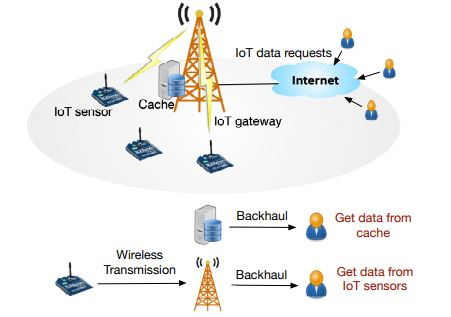
\includegraphics[width=8cm]{systemmodel}}
	\caption{نمایی از سیستم توصیف شده \cite{yao2020caching}}
	\label{fig:systemmodel}
\end{figure}

حال هرکدام از محتویات با یک شناسه‌ی یکتا\footnote{\lr{CID (Content Identifier)}} مشخص می‌گردد. در واقع در هریک از فایل‌ها، شناسه‌ی محتوا، دیتای مربوط به آن (مقدار اندازه گیری شده) به همراه دو برچسب زمانی که یکی بیانگر زمان تولید دیتا یا \lr{$t_{generation}$} و دیگری مدت زمان اعتبار مقدار اندازه‌گیری شده یا به تعبیر ریاضی \lr{$t_{life-time}$} می‌باشد. پارامتر طول عمر دیتا نیز به صورت 
\begin{equation}\label{eq3}
	T_{life} = t_{request} - t_{generation}
\end{equation}
 تعریف می‌شود که از مقایسه‌ی آن با مدت زمان اعتبار دیتا می توان به میزان تازگی دیتا پی برد.

همانطور که پیشتر گفته شد، در هریک از گره‌های لبه یک حافظه‌ی ذخیره‌سای قرار گرفته است. برای واکشی دیتای درخواست‌های ارسالی، در صورتیکه گره لبه محتوای درخواستی را ذخیره نکرده باشد، یک درخواست به گره تولیدکننده‌ی دیتا می‌فرستد و بعد دیتای موردنظر از گره تولیدکننده واکشی می‌شود. سپس گره لبه برای ذخیره یا عدم ذخیره‌ی دیتای به دست آمده یا اینکه آیا نیاز به جایگزینی محتوا در حافظه‌ی کش وجود دارد یا نه، تصمیم می‌گیرد و دیتا را برای کاربر می‌فرستد. حال اگر دیتای درخواست شده در حافظه‌ی کش وجود داشته باشد اما تازه نباشد یا به تعبیر ریاضی \lr{$t_{age} >= t_{life}$} باشد، آنگاه گره لبه برای آپدیت دیتا به گره تولیدکننده درخواست ارسال می‌نماید و پاسخ را برای گره مصرف‌کننده نیز می‌فرستد و مقدار قبلی دیتا را با مقدار جدید جایگزین می‌نماید. حال اگر دیتای درخواست شده در حافظه‌ی کش هنوز معتبر باشد یا به تعبیر ریاضی \lr{$t_{age} < t_{life}$} باشد، آنگاه گره لبه پاسخ را برای گره مصرف‌کننده می‌فرستد و بدین صورت از ارتباط مستقیم با حسگر برای واکشی جواب جلوگیری نمودیم و بنابراین مصرف انرژی حسگر کاهش یافته و حتی نیز با میزان تأخیر کمتری دیتای درخواستی برای گره مصرف‌کننده ارسال می‌گردد. سناریوی توصیف شده را در شکل \ref{fig:simplescenario} مشاهده می‌کنید.
\begin{figure}[ht]
	\centerline{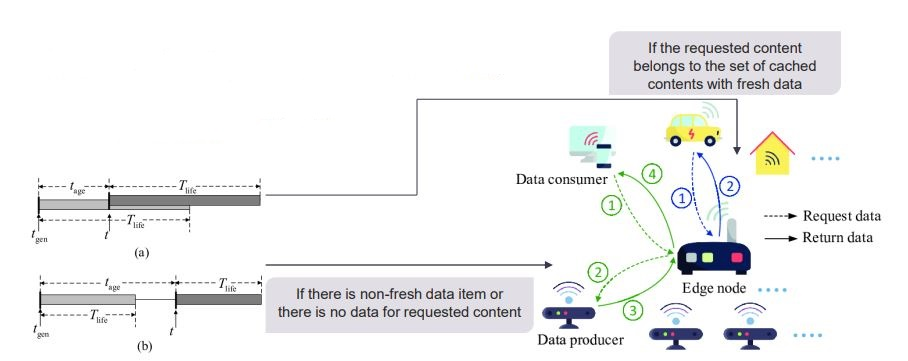
\includegraphics[width=15cm]{simplescenario}}
	\caption{سناریوی واکشی پاسخ در ذخیره‌سازی لبه برای شبکه‌های اینترنت اشیا\cite{cachingtransientdata2018}}
	\label{fig:simplescenario}
\end{figure}

\newpage
\subsection{آشنایی با نمادها و ادبیات یادگیری تقویتی به کار رفته در مسئله}
در این بخش توضیحاتی درباره‌ی نمادگذاری به کار رفته برای بیان ریاضی مسئله ارائه می‌گردد که این بیان در بین مقالات مرور شده در فصل دوم مشترک است.  مجموعه‌ی دیتای ذخیره شده در هر گره لبه در لحظه‌ی \lr{$t_k$} به صورت مجموعه‌ی 
\begin{equation}\label{eq4}
	D_k = \{d_k^1, d_k^2, ..., d_k^I\}
\end{equation}
 مشخص می‌شود. هر کدام از داده‌های ذخیره شده، گزارشی از مقدار یکی از محتویات موجود در شبکه می‌باشد که مجموعه‌ی این محتویات به صورت 
\begin{equation}\label{eq5}
	F_k = \{f_k^1, f_k^2, ..., f_k^I\}
\end{equation}
بیان می‌شود و تناظر یک به یک میان محتویات و دیتای اندازه گیری شده‌ی متناسب با هرکدام به کمک تابع 
\begin{equation}\label{eq6}
	d_k^i = p(f_k^i)
\end{equation}
 تعریف می‌گردد و مقدار \lr{I} برابر با حداکثر تعداد فایل‌هایی است که می‌توان در حافظه‌ی کش ذخیره‌سازی کرد. عامل در گره لبه برای تشخیص تازگی دیتای ذخیره شده نیز به صورت رابطه‌ی \ref{eq:7} عمل می‌نماید.
 \begin{equation}\label{eq:7}
 	d_k = \begin{cases}
 		p(f_k) \text{\lr{ if $f_k \in F_k, t_{age}(p(f_k)) < T_{life}(p(f_k))$}}\\
 		\text{\lr{new item, o.w.}}
 	\end{cases}
 \end{equation}

مفهوم تابع هزینه\footnote{\lr{cost function}} نیز برپایه‌ی هزینه‌ی از دست رفتن تازگی دیتای\footnote{\lr{freshness loss}} ذخیره شده و نیز هزینه‌ی ارتباط\footnote{\lr{communication loss}} برای واکشی پاسخ از حسگر یا حافظه‌ی اختصاص یافته در گره لبه درصورت موجود بودن دیتای درخواستی، مطابق رابطه‌ی\ref{eq:8} تعریف می‌شود. در اینجا \lr{$c_2 > c_1$} است.
\begin{equation}\label{eq:8}
	c(d_k) = \begin{cases}
		c_1 \text{\lr{ if $f_k \in F_k, t_{age}(p(f_k)) < T_{life}(p(f_k))$}}\\
		c_2 \text{\lr{ o.w.}}
	\end{cases}
\end{equation}  
 
 تابع هزینه‌ی مربوط به از دست رفتن اعتبار دیتا به صورت رابطه‌ی\ref{eq:9} تعریف می‌شود که تنها در حالتی که دیتای درخواستی در حافظه موجود و معتبر یاشد، مقدار دارد زیرا که در سایر حالات دیتای معتبر از گره تولیدکننده‌ی مربوطه واکشی می‌گردد و در نتیجه مدت زیادی از زمان تولید آن نگذشته است. 
 \begin{equation}\label{eq:9}
 	l(d_k) = \begin{cases}
 		\frac{t_{age}(p(f_k))}{T_{life}(p(f_k))} \text{\lr{ if $f_k \in F_k, t_{age}(p(f_k)) < T_{life}(p(f_k))$}}\\
 		0 \text{\lr{ o.w.}}
 	\end{cases}
 \end{equation}  
  در نهایت نیز تابع هزینه به صورت میانگین وزن‌دار هزینه‌ی ارتباط و هزینه ی از دست رفتن اعتبار دیتا تعریف می‌شود:
  \begin{equation}\label{eq:10}
  	C(d_k) = \alpha . c(d_k) + (1 - \alpha) . l(d_k)
  \end{equation}

و تابع سودمندی\footnote{\lr{utility function}}، مفهومی در برابر تابع هزینه بوده و به صورت نمایش داده شده در رابطه‌ی\ref{eq:11} مشخص می‌گردد.
\begin{equation}\label{eq:11}
	U(d_k) = B - C(d_k)
\end{equation}

در رابطه‌ی \ref{eq:11} معمولاً مقدار \lr{B} به صورتی تعریف می‌شود که تابع سودمندی به صورت نمایش داده شده در آید:
\begin{equation}\label{eq:12}
	U(d_k) = \alpha . (c_2 - c(d_k)) + (1 - \alpha) . g(d_k)
\end{equation}

در رابطه‌ی \ref{eq:12} منظور از تابع \lr{g(d)} تازگی دیتاست، که به صورت 
\begin{equation}\label{eq:13}
	g(d) = \frac{T_{life}(p(f_k)) - t_{age}(p(f_k))}{T_{life}(p(f_k))} 
\end{equation}  
تعریف می‌شود.

فضای حالات برای جایگزینی محتوا در حافظه براساس محتویات داخل حافظه، دیتای مربوط به هریک از آنها و نیز میزان تازگی یا اعتبار دیتای ذخیره شده، تعیین می‌شود. (این مقادیر حداقل اطلاعات مورد نیاز برای تعیین حالت عامل است. در حالتی که گره‌ها متحرک هستند برای تعیین حالت اطلاعات بیشتری مورد نیاز خواهد بود که در مقالات فصل دوم درباره‌ی آنها بیشتر بحث می‌شود.) با توجه به اینکه میزان اعتبار دیتا به صورت رابطه‌ی \ref{eq:13} به دست می‌آید می توان گفت که فضای حالات در مسئله‌ی ما پیوسته است. 

به طور کلی در صورتی که از گنجایش حافظه‌ی ذخیره‌سازی باقی مانده باشد هر فایل درخواستی که از حسگر واکشی می‌شود در آن ذخیره می‌گردد. حال اگر حافظه‌ی ذخیره‌سازی پر شود، فایل با محبوبیت کمتر از حافظه حذف شده و جای خود را به فایل جدید می‌دهد. حال اگر فایل درخواستی در حافظه موجود باشد ولی اعتبار خود را از دست داده باشد دوباره نیاز داریم تا داده‌ی معتبر را از گره تولیدکنده ی مربوطه واکشی نماییم و دیتای مربوط به آن به روز رسانی می‌شود. اکشن‌های توصیف شده در حالات مختلف فضای اکشن‌ها را برای ما مشخص می‌نماید و اینکه در شرایط مختلف چه عملی بهینه تلقی می‌گردد، سیاست بهینه را برای ما مشخص می‌سازد. حال محیط پاداشی را پس از اعمال اکشن اتخاذ شده به عامل می‌دهد و حال اینکه توزیع پاداش به چه صورت باید باشد یا به عبارتی چگونگی شبیه‌سازی آن در مسئله‌ سوال مهمی است که پیاده‌سازی متفاوتی برای آن در مقالات انجام شده است. 
 
 حال در  مقالاتی که در فصل دوم ارائه می‌گردد، تفاوت در الگوریتم‌های به کار رفته برای تخمین ارزش استیت‌ها ارزش استیت-اکشن‌ها یا حتی سیاست بهینه می‌باشد. در بعضی نیز بنا به شرایط محیطی، پارامترهایی برای تعیین استیت به مسئله اضافه می‌شود یا در برخی دیگر از الگوریتم‌های یادگیری عمیق سلسله مراتبی\footnote{\lr{Hierarchical Deep Reinforcement Learning}} برای تعیین سیاست جایگزینی محتوا در حافظه استفاده می‌شود که این به معنی استفاده از یک استراتژی جدید مبنی بر قرار دادن حافظه‌ی ذخیره‌سازی در گره‌های لبه و یک لایه دورتر از گره‌های مصرف‌کننده (اصطلاحاً معماری ریشه-برگ\footnote{\lr{parent-leaf architecture}}) می‌باشد.

\section{جمع بندی}
به طور کلی دو ویژگی منحصربفرد شبکه‌های اینترنت اشیا یکی محدودیت سطح انرژی حسگرها و دیگری محدودیت مدت زمان اعتبار دیتا، مسئله‌ی ذخیره‌سازی در این شبکه‌ها را در مقایسه با استراتژی ذخیره‌سازی در سایر شبکه های مبتنی بر محتوا متمایز می‌سازد. علاوه براین با توجه به غیرایستان بودن محبوبیت فایل‌ها در طول زمان، به کارگیری یک استراتژی مبتنی بر یادگیری تقویتی عمیق برای جایگزینی محتوا در حافظه‌ی ذخیره‌سازی با توجه به محدودیت گنجایش آن، می‌تواند زمان لازم برای واکشی پاسخ را کاهش داده و نیز ترافیک شبکه را متوازن‌تر نماید و در نتیجه‌ی آن مصرف انرژی حسگر یا گره تولیدکننده‌ی داده کاهش می‌یابد. فصل دوم نیز به مرور مقالات مطالعه شده اختصاص یافته است.





